\newpage
\section{Look up table}

A look up table is a table for looking up some predefined values. In the AU2 it's used for looking up a power for a specificity speed. It a 2D-LUT because there is a table for the car when it is accelerating and a table when the car has met the required speed. The second table will normally not been used, because the coast and burn will normal be activated then the last table are in use. The look up table are build from the efficiency diagram figure \ref{fig:eff_maxon_36V}. 

\begin{figure}[H]
	\centering
	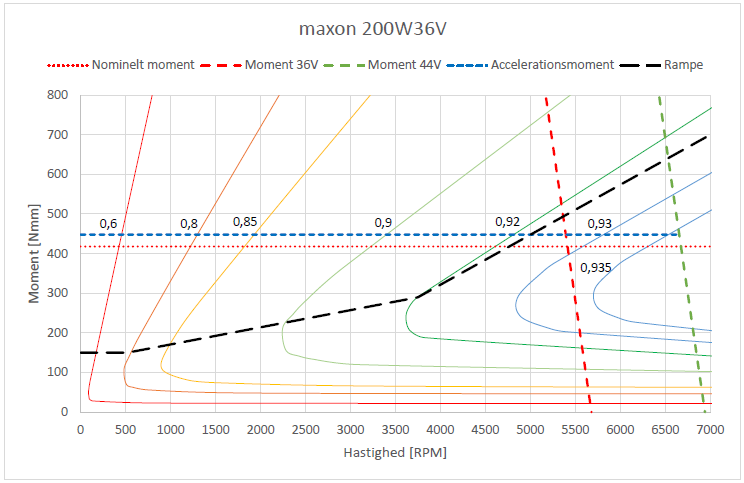
\includegraphics [width=4in]{Software/Pictures/maxon-200W36V.PNG}
	\caption{Efficiency diagram - maxon 200W36V. From AU2 M7BAC\_Optimering af drivlinje}
	\label{fig:eff_maxon_36V}
\end{figure}

The diagram show where the efficiency is best, and ramp to hit the best efficiency and lowest power consuming. Too see have the ramps are calculate see "AU2 M7BAC\_Optimering af drivlinje"\cite{BAC_zenith33} the different ramp that are calculated is listed here figure \ref{fig:eff_maxon_36V_ramp1-3} \& \ref{fig:eff_maxon_36V_ramp4-6}.

\begin{figure}[H]
	\centering
	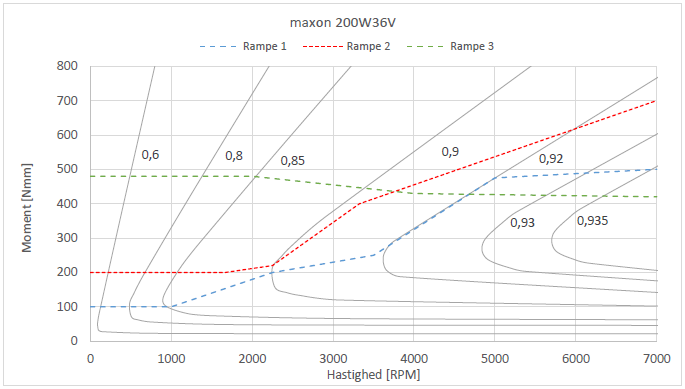
\includegraphics [width=4in]{Software/Pictures/Momentramper-1-3.PNG}
	\caption{Efficiency diagram - maxon 200W36V - ramp 1 to 3. From AU2 M7BAC\_Optimering af drivlinje}
	\label{fig:eff_maxon_36V_ramp1-3}
\end{figure}

\begin{figure}[H]
	\centering
	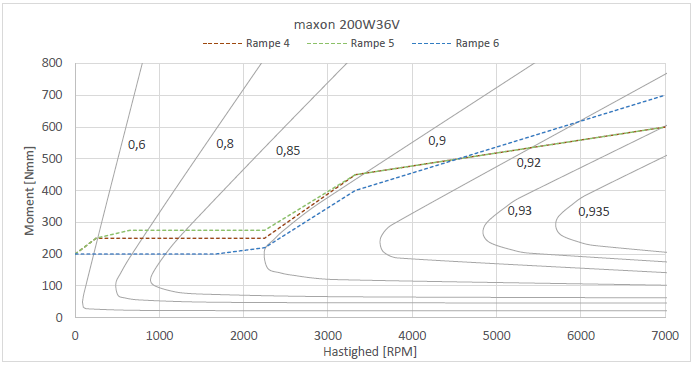
\includegraphics [width=4in]{Software/Pictures/Momentramper-4-6.PNG}
	\caption{Efficiency diagram - maxon 200W36V - ramp 4 to 6. From AU2 M7BAC\_Optimering af drivlinje}
	\label{fig:eff_maxon_36V_ramp4-6}
\end{figure}

The power consuming of the ramps are listing here. The power consuming over the time it takes them to hit the wanted speed. figure \ref{fig:eff_maxon_36V_ramp_energy-consumption}.

\begin{figure}[H]
	\centering
	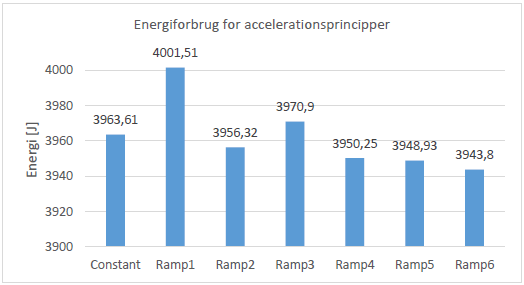
\includegraphics [width=4in]{Software/Pictures/energy-consumption.PNG}
	\caption{Energy consumption- maxon 200W36V - ramp 1 to 6. From AU2 M7BAC\_Optimering af drivlinje}
	\label{fig:eff_maxon_36V_ramp_energy-consumption}
\end{figure}

On the first look at \ref{fig:eff_maxon_36V_ramp_energy-consumption} it seems like the best choice would be ramp 6, but  this ramp has a power peak at $ \SI{450}{\watt} $! The motor limit is $ \SI{200}{\watt} $. 

\begin{equation}
	\begin{split}
		\omega_{AU2_{max}} = \SI{6600}{rpm}\\
		T_{ramp6_{max}} = \SI{650}{\newton \milli\metre} \\
		P_{ramp6_{max}} = \omega_{AU2_{max}} \times T_{ramp6_{max}} = \SI{450}{\watt}
	\end{split}
\end{equation}

To find out what ramp to use, the ramp must not exceed the power limit \ref{fig:eff_maxon_36V_Power_limit} and have the lowest energy consumption. The ramp 5 are choose but it exceed the power limit a little.

\begin{figure}[H]
	\centering
	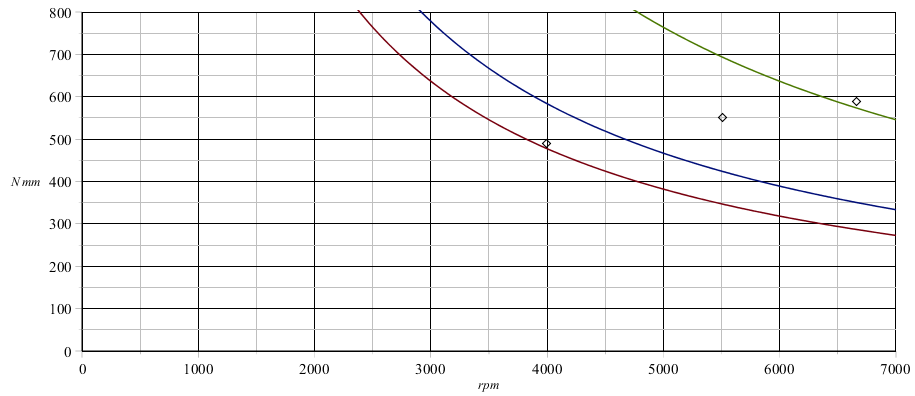
\includegraphics [width=4in]{Software/Pictures/Power_limit.PNG}
	\caption{Power limit - maxon 200W36V. red line 200 Watt @ 36V. blue line 244 Watt @ 44 V (over power). Green line 400 watt}
	\label{fig:eff_maxon_36V_Power_limit}
\end{figure}

\subsubsection{Calculation script - LUT}

The ramp and only needs to be converted to the PSoC that controls the Motor. To this a Matlab script has been made, where it just insert the motors Max-power and -peak power. Gear setup and max speed.    
\lstset{language=matlab}
\begin{lstlisting}
%% insert values
FILE_NAME='src\MotorController.cydsn\LUT_data.h';

H_d=0.478;
gear=1/20;
MAX_Watt = 200;
MAX_Watt_peak = 300;
MAX_speed = 8.34;

% ex. ramp = [Nmm rpm efficiency; ...]
ramp = [200 0 0.5; 250 250 0.6; 250 2250 0.8; 450 3300 0.85; 600 7000 0.9];
const = [0 0 0.5; 50 100 0.6; 110 500 0.8; 110 900 0.85; 220 2250 0.9; 250 3600 0.92; 275 4800 0.93; 295 5600 0.935];

% calculation
...

\end{lstlisting}

The result from the script are plotted here \ref{fig:LUT_plot}. 

\begin{figure}[H]
	\centering
	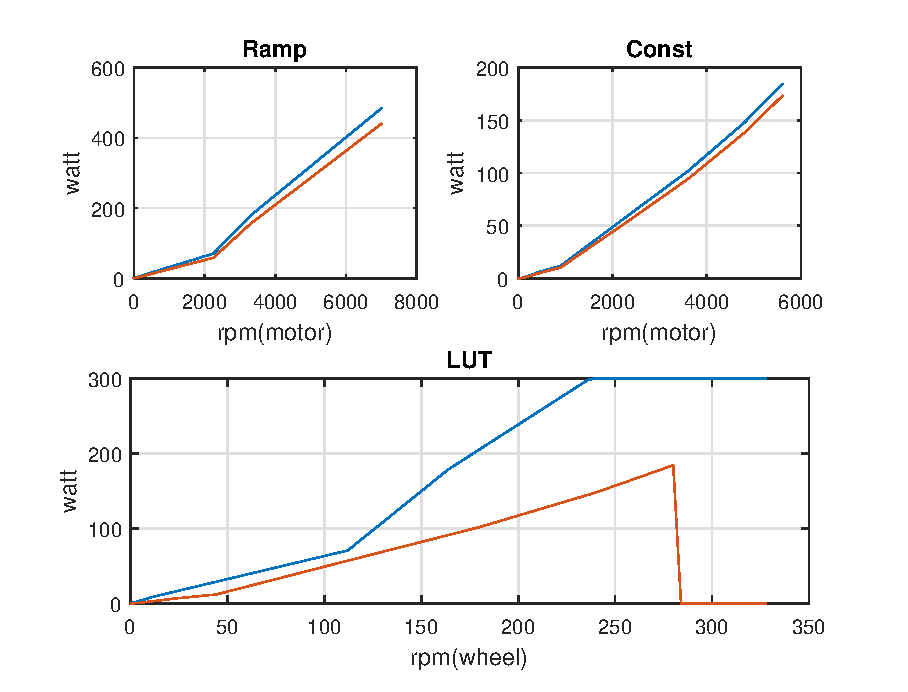
\includegraphics [width=6in]{Software/Pictures/LUT.eps}
	\caption{LUT plot - "Ramp" is the power use for a specific speed(red = without power loose, blue = with power loose) this table are used then accelerating. "Const" is the same but just then the car should hold a constant speed(red = without power loose, blue = with power loose). "LUT" is the 2D-look Up Table(blue = accelerating; red constant speed)}
	\label{fig:LUT_plot}
\end{figure}

This is then automatic moved into the PSoC creator as a header-file, what is generated by the script. Where are build a small class to handle the LUT.
It will first see if the speed is equal or grater then the wanted speed so it knows that LUT to use. Now it will look up a power value what match the speed and return a new wanted power value.



